\documentclass[]{article}
\usepackage{lmodern}
\usepackage{amssymb,amsmath}
\usepackage{ifxetex,ifluatex}
\usepackage{lscape}
\usepackage[demo]{graphicx}
\usepackage{floatrow}
\usepackage{fixltx2e} % provides \textsubscript
\ifnum 0\ifxetex 1\fi\ifluatex 1\fi=0 % if pdftex
  \usepackage[T1]{fontenc}
  \usepackage[utf8]{inputenc}
\else % if luatex or xelatex
  \ifxetex
    \usepackage{mathspec}
  \else
    \usepackage{fontspec}
  \fi
  \defaultfontfeatures{Ligatures=TeX,Scale=MatchLowercase}
\fi
% use upquote if available, for straight quotes in verbatim environments
\IfFileExists{upquote.sty}{\usepackage{upquote}}{}
% use microtype if available
\IfFileExists{microtype.sty}{%
\usepackage{microtype}
\UseMicrotypeSet[protrusion]{basicmath} % disable protrusion for tt fonts
}{}
\usepackage[margin=1in]{geometry}
\usepackage{hyperref}
\hypersetup{unicode=true,
            pdftitle={PREPRINT: Using digital epidemiology methods to monitor influenza-like illness in the Netherlands in real-time: the 2017-2018 season},
            pdfborder={0 0 0},
            breaklinks=true}
\urlstyle{same}  % don't use monospace font for urls
\usepackage{graphicx,grffile}
\makeatletter
\def\maxwidth{\ifdim\Gin@nat@width>\linewidth\linewidth\else\Gin@nat@width\fi}
\def\maxheight{\ifdim\Gin@nat@height>\textheight\textheight\else\Gin@nat@height\fi}
\makeatother
% Scale images if necessary, so that they will not overflow the page
% margins by default, and it is still possible to overwrite the defaults
% using explicit options in \includegraphics[width, height, ...]{}
\setkeys{Gin}{width=\maxwidth,height=\maxheight,keepaspectratio}
\IfFileExists{parskip.sty}{%
\usepackage{parskip}
}{% else
\setlength{\parindent}{0pt}
\setlength{\parskip}{6pt plus 2pt minus 1pt}
}
\setlength{\emergencystretch}{3em}  % prevent overfull lines
\providecommand{\tightlist}{%
  \setlength{\itemsep}{0pt}\setlength{\parskip}{0pt}}
\setcounter{secnumdepth}{0}
% Redefines (sub)paragraphs to behave more like sections
\ifx\paragraph\undefined\else
\let\oldparagraph\paragraph
\renewcommand{\paragraph}[1]{\oldparagraph{#1}\mbox{}}
\fi
\ifx\subparagraph\undefined\else
\let\oldsubparagraph\subparagraph
\renewcommand{\subparagraph}[1]{\oldsubparagraph{#1}\mbox{}}
\fi

%%% Use protect on footnotes to avoid problems with footnotes in titles
\let\rmarkdownfootnote\footnote%
\def\footnote{\protect\rmarkdownfootnote}

%%% Change title format to be more compact
\usepackage{titling}

% Create subtitle command for use in maketitle
\newcommand{\subtitle}[1]{
  \posttitle{
    \begin{center}\large#1\end{center}
    }
}

\setlength{\droptitle}{-2em}
  \title{PREPRINT: Using digital epidemiology methods to monitor influenza-like illness in
the Netherlands in real-time: the 2017-2018 season}
  \pretitle{\vspace{\droptitle}\centering\huge}
  \posttitle{\par}
  \author{}
  \preauthor{}\postauthor{}
  \date{}
  \predate{}\postdate{}

\usepackage{booktabs}
\usepackage{fancyhdr}
\pagestyle{fancy}

\lhead{Preprint: Schneider, et al. 'Dutch Flu Trends'. 2018}


\begin{document}
\maketitle

\bigskip

\textbf{Schneider PP\textsuperscript{1,2}, van Gool
CJAW\textsuperscript{3}, Spreeuwenberg P\textsuperscript{2}, Hooiveld
M\textsuperscript{2}, Donker GA\textsuperscript{2}, Barnett
DJ\textsuperscript{1}, Paget J\textsuperscript{2}}

\begingroup\small

\emph{\textsuperscript{1} Faculty of Health, Medicine and Life Sciences,
Maastricht University, \textsuperscript{2} Nivel (Netherlands Institute
of Health Service Research), \textsuperscript{3} School CAPHRI,
Maastricht University}

Contact:
\href{mailto:project.flutrend@gmail.com}{\nolinkurl{project.flutrend@gmail.com}}
\endgroup

\bigskip

\hypertarget{abstract}{%
\subsection{\texorpdfstring{\textbf{Abstract}}{Abstract}}\label{abstract}}

\textbf{Introduction}\\
Despite the early development of Google Flu Trends in 2009, digital
epidemiology methods have not been adopted widely, with most research
focusing on the USA. In this article we demonstrate the prediction of
real-time trends in influenza-like illness (ILI) in the Netherlands
using search engine query data.

\textbf{Methods}\\
We used flu-related search query data from Google Trends in combination
with traditional surveillance data from 40 general sentinel practices to
build our predictive models. We introduced an artificial 4-week delay in
the use of GP data in the models, in order to test the predictive
performance of the search engine data.

Simulating the weekly use of a prediction model across the 2017/2018 flu
season we used lasso regression to fit 52 prediction models (one for
each week) for weekly ILI incidence. We used rolling forecast
cross-validation for lambda optimization in each model, minimizing the
maximum absolute error.

\textbf{Results}\\
The models accurately predicted the number of ILI cases during the
2017/18 ILI epidemic in real time with a mean absolute error of 1.40
(per 10,000 population) and a maximum absolute error of 6.36. The model
would also have identified the onset, peak, and end of the epidemic with
reasonable accuracy

The number of predictors that were retained in the prediction models was
small, ranging from 3 to 5, with a single keyword (`Griep' = `Flu')
having by far the most weight in all models.

\textbf{Discussion}\\
This study demonstrates the feasibility of accurate real-time ILI
incidence predictions in the Netherlands using internet search query
data .Digital ILI monitoring strategies may be useful in countries with
poor surveillance systems, or for monitoring emergent diseases,
including influenza pandemics. We hope that this transparent and
accessible case study inspires and supports further developments in
field of digital epidemiology in Europe and beyond.

\bigskip

\begin{center}\rule{0.5\linewidth}{\linethickness}\end{center}

\newpage

\hypertarget{introduction}{%
\subsection{\texorpdfstring{\textbf{Introduction}}{Introduction}}\label{introduction}}

Previous studies suggest that traditional disease surveillance systems
could be complemented with information from online data
sources.{[}1--3{]} The underlying premise is that people, nowadays,
often turn to the internet when they face health problems.{[}4{]} With
influenza-like illness (ILI), individuals might search for information
about symptoms, look for remedies, or share messages on social media.
All of these interactions leave digital footprints, which, when
aggregated, could be harnessed to monitor disease activity.{[}1{]} In
this way, online data streams could be used to support the timely
detection of infectious disease outbreaks.

This hypothesis is not new, and in 2009 researchers at Google reported
that their `Flu Trends' model was able to predict ILI activity in the
United States in real-time, by monitoring millions of queries on their
search engine.{[}5{]} The aim of Google Flu Trends was to bridge a
two-week lag in the reporting of ILI cases in the official surveillance
statistics. Initially, the project indeed appeared to provide accurate
predictions and was expanded to cover 29 countries around the world. In
2012, however, the model's performance deteriorated, and in early 2013,
it overestimated the peak of the epidemic by more than 140\%. The
failure, and subsequent termination of Google Flu Trends, received a lot
of media attention and it also sparked an intense debate about the
limitations of `big data' in epidemiological research.{[}3,6{]}

Since then, the number of scholarly articles published in the field of
digital epidemiology has grown significantly.{[}2,7{]} The discipline
is, nevertheless, in an early stage and should still be considered as
being experimental. Especially outside of the United States, there has
been little effort to investigate the value of online data sources for
epidemiological purposes.

Building on previous work,{[}8{]} our study assesses whether online
search queries can be used to predict the ILI epidemic in the
Netherlands during the 2017-2018 winter in real-time. Our investigation
is meant to be an accessible case study in digital epidemiology. The
full source code and data are provided under open license to encourage
the application of this method to other countries and to other areas of
epidemiological research.

\hypertarget{methodology}{%
\subsection{\texorpdfstring{\textbf{Methodology}}{Methodology}}\label{methodology}}

\hypertarget{ili-data}{%
\subsubsection{\texorpdfstring{\textbf{ILI-data}}{ILI-data}}\label{ili-data}}

Weekly data on consultations for ILI were collected through sentinel
practices participanting in the Nivel Primary Care Database,{[}9{]}, and
released by the European Centre for Disease Prevention and
Control.{[}10{]} The practices constitute a nationally representative
group of 40 general practices in the Netherlands. The methodology is
further described by Donker.{[}11{]} It is important to note that the
data are available in real-time and that the four-week reporting lag
that we have assumed in this paper was only simulated for the purpose of
our study.

\hypertarget{web-search-queries}{%
\subsubsection{\texorpdfstring{\textbf{Web search
queries}}{Web search queries}}\label{web-search-queries}}

Data on web search queries were retrieved from Google Trends{[}12{]}.
This online service provides statistics on how often a particular
keyword was searched relative to the total search-volume across various
regions of the world. It also provides information on related search
queries (``people who searched for this, also searched for that'').

To identify potentially relevant keywords for our study, we retrieved
the 25 terms that were most related to the search term `griep', the
Dutch word for `flu'. All keywords that contained a year were excluded,
because they were - a priori - expected to be poor predictors of ILI
rates in other years. Further a priori filtering of search terms wasnot
performed. For the remaining search terms, we used the R-package
gtrendsR{[}13{]} to download five years of weekly query statistics (from
week 33/2013 to week 31/2018) for the Netherlands from Google Trends.
Subsequently, we expanded the set of predictors by multiplying each
predictor with all other predictors (to account for one-level
interactions) and with themselves (to account for non-linearities).

\hypertarget{modeling}{%
\subsubsection{\texorpdfstring{\textbf{Modeling}}{Modeling}}\label{modeling}}

We simulated the weekly use of a statistical model for predicting ILI
incidence rates in real-time, based on Google search query statistics,
during the 2017/18 ILI epidemic in the Netherlands. We assumed a
four-week delay between the identification and the reporting of ILI
cases, so that at week \(w\), the ILI incidence of week \(w-4\) became
available. For each week, the model was updated and re-fitted with the
most recently available information (the search query data up until the
current week), and the ILI incidence data up until four weeks ago. The
updated model was then used to predict the ILI incidence for the current
and the previous three weeks (i.e.~to fill the assumed four-week
reporting lag). To account for the temporal structure of the analysis,
we set up an automated loop that iteratively splits the data into
training and validation sets. The training data was used to fit a
prediction model and the validation set was used to evaluate the model's
predictions on new data points.

\hypertarget{automated-analysis-loop}{%
\subsubsection{\texorpdfstring{\textbf{Automated analysis
loop}}{Automated analysis loop}}\label{automated-analysis-loop}}

The first four years of data (week 33/2013 to 30/2017) were used as
training data only, while the analysis loop was run on the \(52\) weeks
of the influenza season 2017/2018 (week 31/2017 to 31/2018). At each
week, the data were split into a training set (for which both the ILI
and Google data were made available to the model) and a four week
validation set (for which only Google data were made available). This
means, at the \(ith\) iteration of the loop, the analysis contained
\(207 + i\) weeks of training data (week 1 to \(207 + i\)), and 4 weeks
of validation data (week \(207 + i + 1\) to \(207 + i + 4\)). Each week,
a new model was built to predict the ILI incidence of the current week
and the previous three weeks.

The model building process included the following steps. Firstly,
dependent and independent variables were normalized and centered, with a
mean of zero. This was performed separately for training and validation
data, to prevent information leaking from the validation set. Variables
with near zero variance were removed. We then used lasso (least absolute
shrinkage and selection operator) regression,{[}14{]} in combination
with cross validation (CV), to determine the optimal set of predictors
and their regularized coefficients. See Technical Appendix (and the
provided source code) for a detailed outline of the methods.

Lasso regression performs simultaneous variable selection and
coefficient estimation. It imposes a penalty on the absolute values of
the coefficients in the least squares estimation. In effect, less
important parameters shrink towards zero, resulting in a selection of
predictors, if coefficients become zero. The model's complexity is
controlled by the penalty parameter \(\lambda\). Rolling forecast CV for
time series, with fixed origin and expanding window, was used to find
the optimal value for \(\lambda\).

CV for time series is a variation of leave-k-out CV, which can be used
to avoid the leakage of information from future to past observations.
Similar to our automated analysis loop, CV for time series splits the
data iteratively into a training set (the first \(k\) weeks) and a test
or `hold-out' set (the subsequent \(4\) weeks). In the first CV
iteration, a lasso regression model is fit on data from week 1 to
\(k = 52\) and its predictions are tested on hold-out data from week 53
to 56. The process then `rolls' forward, week-by-week, keeping the
origin at week 1, and using an expanding number of weeks as training
data with \(k = 52+1, +2,...,+m\), whereby \(m\) increases with each
iteration \(i\) of the outer analysis loop, with \(m = 207 - 52 + i\).
The prediction error over all \(m\) four-week hold-out sets is then
aggregated to assess how well the statistical model can predict new data
points. At each iteration of the outer analysis loop, the inner CV loop
is run for 100 values of the penalty parameter \(\lambda\), (ranging
from \(10^{-8}\) to \(10^{1/4}\)).

The \(\lambda_i\) of the model with the lowest maximum absolute error in
the CV hold-out sets was used to fit the \(ith\) final lasso regression
model on \(207 + i\) weeks of training data, and to predict the ILI
incidence for weeks 1-4 of the \(ith\) validation set. We used the
\emph{maximum} instead of the more commonly used \emph{mean} absolute
error as the selection criterion to increase model stability.

\hypertarget{model-evaluation}{%
\subsubsection{\texorpdfstring{\textbf{Model
evaluation}}{Model evaluation}}\label{model-evaluation}}

We analyzed the predictions of 52 lasso regression models (one for each
week of year 5). Each model provided four predicted values,
corresponding to the four weeks of the validation sets (except the
first/last three models which had shorter horizons). We refer to the
prediction of the current week as week 4 prediction (= 4 weeks since the
last updated with official ILI data), and to the predicted values for
the previous three weeks, as week 3 -1 predictions. Similarly, for all
but the first three weeks of the validation period, there were four
predicted values available.

We plotted the observed against the predicted ILI incidence values and
assessed the performance of the statistical models over the validation
period in terms of the mean absolute error (MAE). The accuracy of the
week 1 - 4 predictions was evaluated separately and all values were
back-transformed to their original scale. For comparison with previous
studies, we also report the Pearson and Spearman correlation
coefficients - however, correlations are not based on the absolute
differences between the predicted and observed values and might,
therefore, generate conflicting or misleading results. We also assessed
how accurately the model predicted the onset and peak of the season.
Furthermore, we investigated which search query terms were retained as
predictors in the 52 models.

\hypertarget{source-code-and-data-availability}{%
\subsubsection{\texorpdfstring{\textbf{Source code and data
availability}}{Source code and data availability}}\label{source-code-and-data-availability}}

The R-code for this study is provided under open CC BY license and the
data that were used for this study can be accessed online.{[}15{]}

\hypertarget{results}{%
\subsection{\texorpdfstring{\textbf{RESULTS}}{RESULTS}}\label{results}}

\hypertarget{google-search-queries}{%
\paragraph{\texorpdfstring{\textbf{Google search
queries}}{Google search queries}}\label{google-search-queries}}

We retrieved information on 26 search terms (`Griep' and the 25 most
related keywords) from Google Trends (see table 1). Six terms were
excluded from the analysis, as they contained a year. For all other
terms (n=20), weekly search query statistics from 2013-08-12 to
2018-08-06 were downloaded. Overall, there was a high correlation
between the query statistics, with an average correlation coefficient of
0.70 (minimum = 0.24; maximum = 0.97). Variables for first-order
interactions between predictors (n = 190) and quadratic terms (n = 20)
were included in the model. Together with the original keywords (n =
20), a total of 230 variables were considered in the analysis as
potential predictors of the ILI incidence.

\begin{table}

\caption{Search terms retrieved from Google Trends}
\centering
\begin{tabular}[t]{lll}
\toprule
Griep & tegen griep & griep wat te doen\\
symptomen & griep 2015* & griep zwanger\\
griep symptomen & griep 2017* & ziek\\
de griep & symptomen griep 2018* & griep spierpijn\\
griep 2018* & griep heerst & hoofdpijn griep\\
\addlinespace
griep koorts & verkoudheid & verschijnselen griep\\
koorts & hoe lang duurt griep & hoofdpijn\\
griep 2016* & heerst er griep & griep nu\\
griep hoe lang & griep 2014* & \\
\bottomrule
\multicolumn{3}{l}{\textsuperscript{*} Terms were removed from further analysis}\\
\end{tabular}
\end{table}

\hypertarget{real-time-ili-incidence-prediction-models}{%
\paragraph{\texorpdfstring{\textbf{Real-time ILI incidence prediction
models}}{Real-time ILI incidence prediction models}}\label{real-time-ili-incidence-prediction-models}}

We simulated the weekly use of a real-time prediction model during the
52 weeks of the 2017/18 ILI season in the Netherlands. At each week, a
new prediction model was built to estimate the ILI incidence of the
current week (week 4) and the previous three weeks (weeks 3-1). Figure 1
shows the values of these week 1-4 predictions separately against the
observed ILI incidence.

Overall, the 52 final lasso regression models predicted the ILI
incidence with reasonable accuracy. The MAE for weeks 1,2,3, and 4 were
1.31, 1.35, 1.38, and 1.40. The corresponding Pearson correlation
coefficients ranged between 0.95and 0.94, and Spearman coefficients were
0.90 for all four weeks.

Before the start of the epidemic in week 50/2017, the error was
generally low, but it increased during the onset, and especially during
the epidemic peak, when the highest prediction error (= 6.36) was
registered (week 10/2018). After week 09-10/2018, the incidence was
underpredicted by the models.

The model's MAE in the validation period was slightly lower than the MAE
observed in the CV hold-out sets (CV MAE for 1,2,3, and 4 predictions
were 1.486, 1.547, 1.625, and 1.676). The maximum absolute error was
markedly lower in the CV hold out sets (1.72).

The bottom plot in Figure 1 provides an overview of the entire five year
observation period. The vertical blue line separates the training (left)
from the validation period (right). For comparative purposes, the
predicted values for the training period of the first prediction model
(run in week 31/2017) are provided (first model training MAE = 1.32;
maximum error 7.18). The figure also illustrates the seasonality of ILI
epidemics (black line). The epidemic in 2017/18 had a slightly higher
intensity and lasted longer than average, but was otherwise not
exceptional.

\begin{landscape}
\begin{figure}
\centering
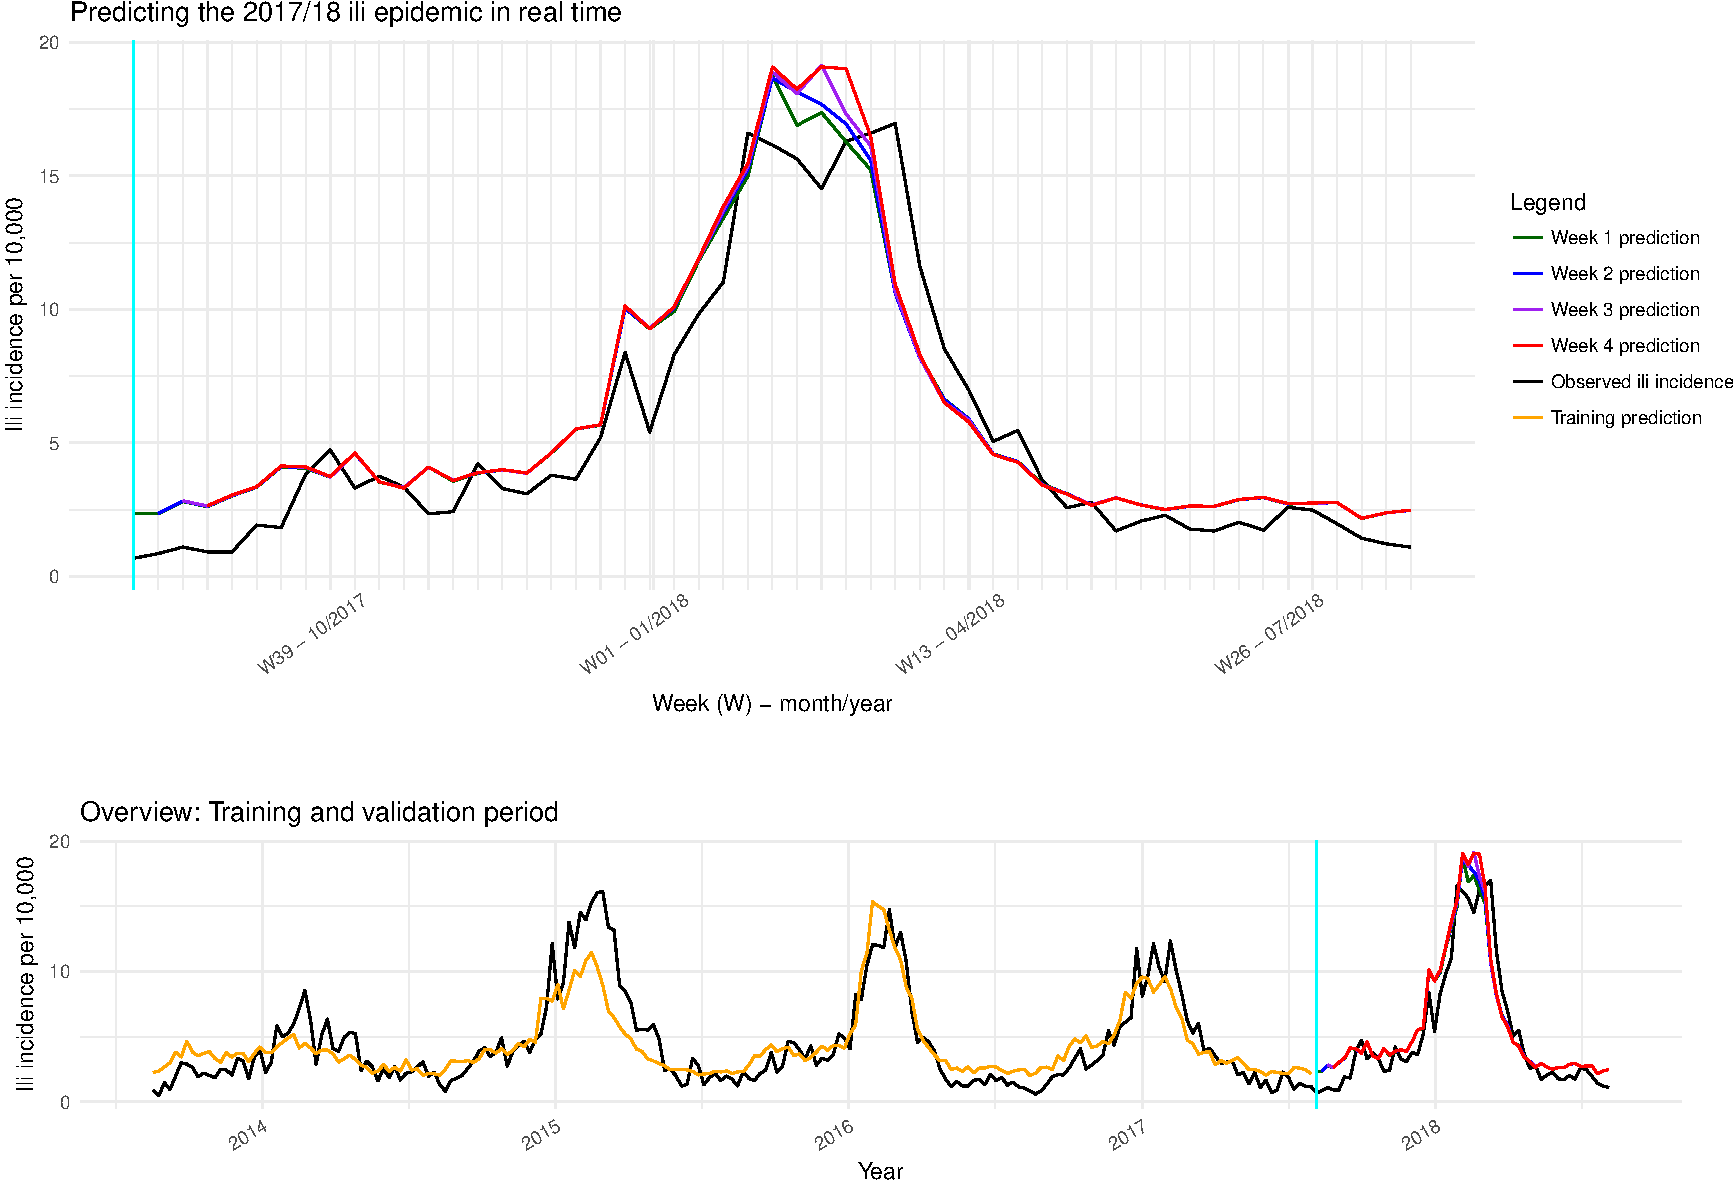
\includegraphics{unnamed-chunk-3-1.pdf}
\caption{The time series plot shows the observed ILI incidence from week
16/2013 to week 15/2018 against the predictions of the 52 final lasso
regression models. For the validation period (top), each model provides
estimates for the week in which it was ran (week 4) and the previous
three weeks (week 3-1). In addition, predicted values within the
training set are provided for the first lasso regression model
(bottom).}
\end{figure}
\end{landscape}

\hypertarget{temporal-aspects-of-ili-incidence-predictions}{%
\paragraph{\texorpdfstring{\textbf{Temporal aspects of ILI incidence
predictions}}{Temporal aspects of ILI incidence predictions}}\label{temporal-aspects-of-ili-incidence-predictions}}

From the visual presentation in Figure 1, it might be difficult to get
assess what information was available at which week. To illustrate the
temporal dynamics of the ILI prediction model, Figure 2 shows the
results of 5 models at different points in time.

The model would have indicated the onset of the season one week ahead of
the sentinel surveillance data (Panel A: observed onset = week 50/2017,
predicted onset = week 49/2017). The peak of the season was predicted in
week 07/2018 (Panel B), while the observed peak was biphasic with the
highest incidence (=16.97) in week 10/2018 and the second highest
(=16.6) in week 04/2018 (Panel C and D). The end of the season (i.e.~ILI
incidence falls below 5.1 per 10,000 for two consecutive weeks) was
predicted in week 14/2018, and observed in week 16/2018 (Panel E).

Visual inspection indicates that the predictions generally appeared to
be ahead of the actual ILI incidence. In fact, throughout the validation
period, week 4 predictions were forecasting the ILI incidence of the
coming week slightly more accurately (MAE = 1.11), than predicting the
current week (MAE = 1.4).


\begin{figure}
\floatbox[{\capbeside\thisfloatsetup{capbesideposition={right,top},capbesidewidth=6cm}}]{figure}[\FBwidth]
{\caption{Observed versus predicted ILI incidence, showing data available at five points during the 2017/18 ILI season. The plots illustrate what information the prediction models would have provided at that particular point in time, if they were used. The y-axis shows the ILI incidence per 10,000 inhabitants; the week for which the last official ILI incidence data were made available is marked by the vertical cyan line; the current week, i.e. the week in which the model is used, is indicated by a red tick mark.}\label{fig:test}}
{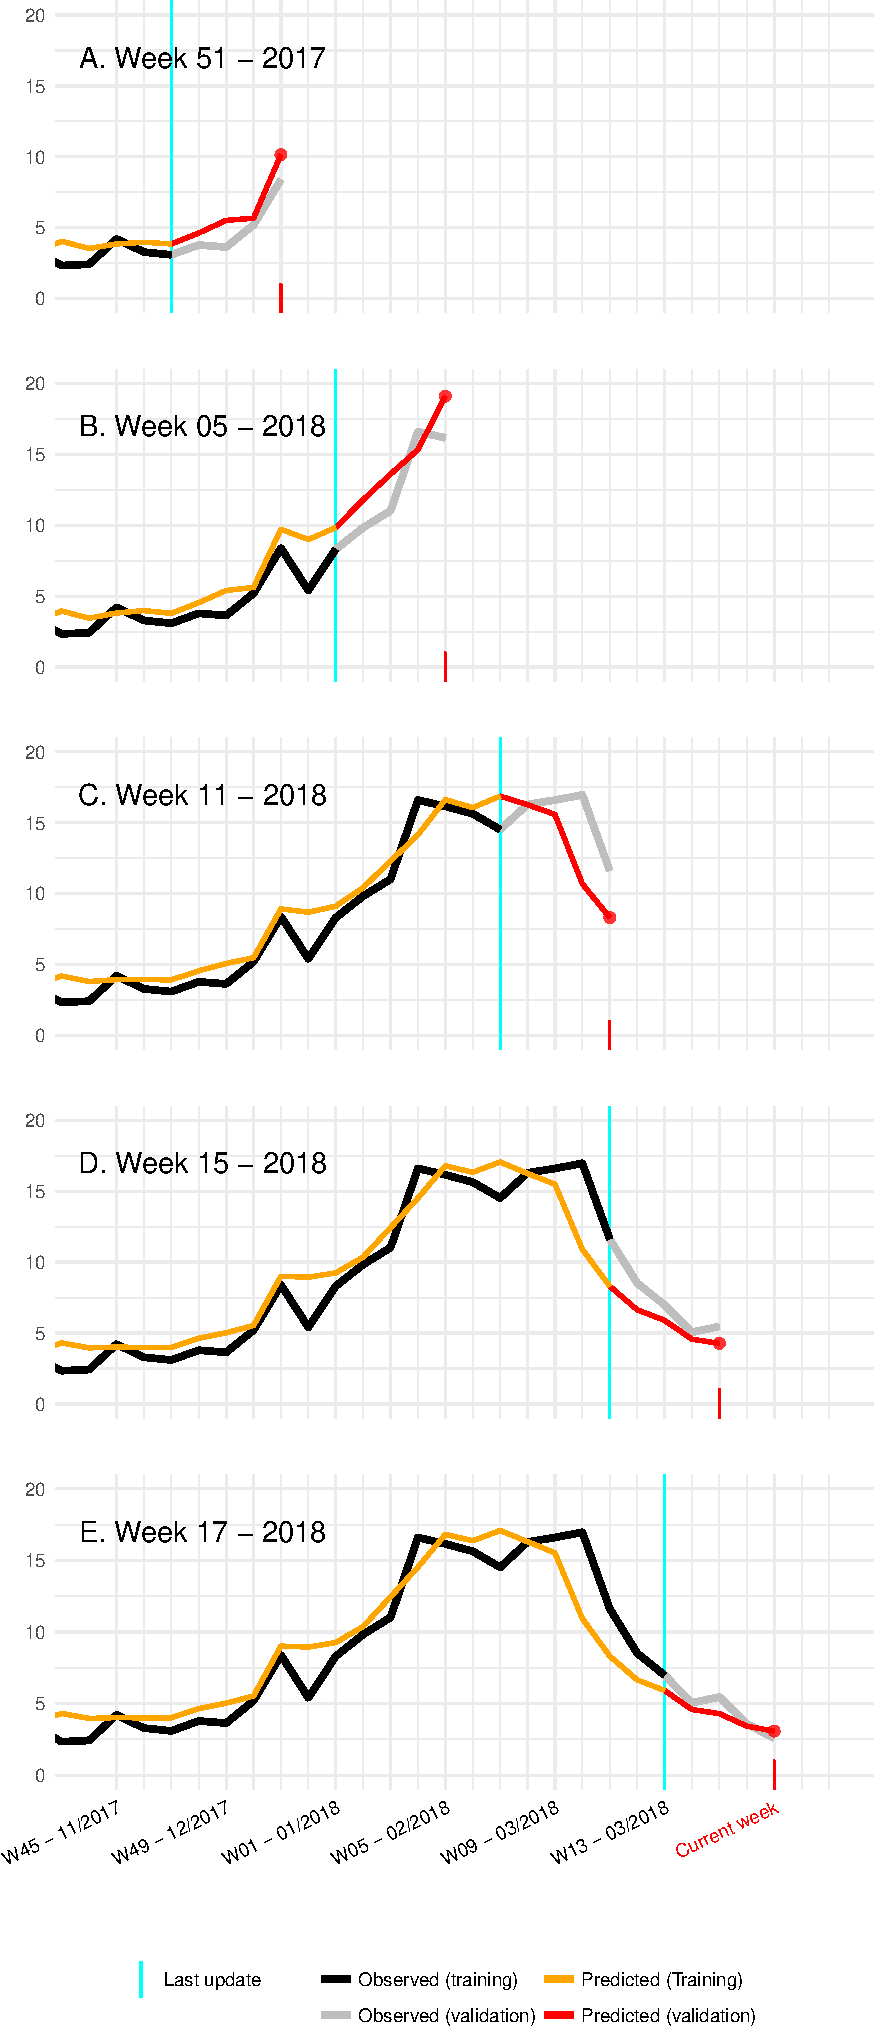
\includegraphics[width=10cm]{unnamed-chunk-4-1}}
\end{figure}




\hypertarget{model-specifications}{%
\paragraph{\texorpdfstring{\textbf{Model
specifications}}{Model specifications}}\label{model-specifications}}

Figure 3 provides an overview of the 52 weekly sets of predictors and
their coefficients used in the final prediction models. During the
validation period, the number of variables that were retained in the
models as predictors ranged from 3 to 5. However, one predictor (`Griep'
= `Flu') had by far the most weight in all models, especially after week
32 of the validation period (= week 11 - 2018).

\begin{figure}
\centering
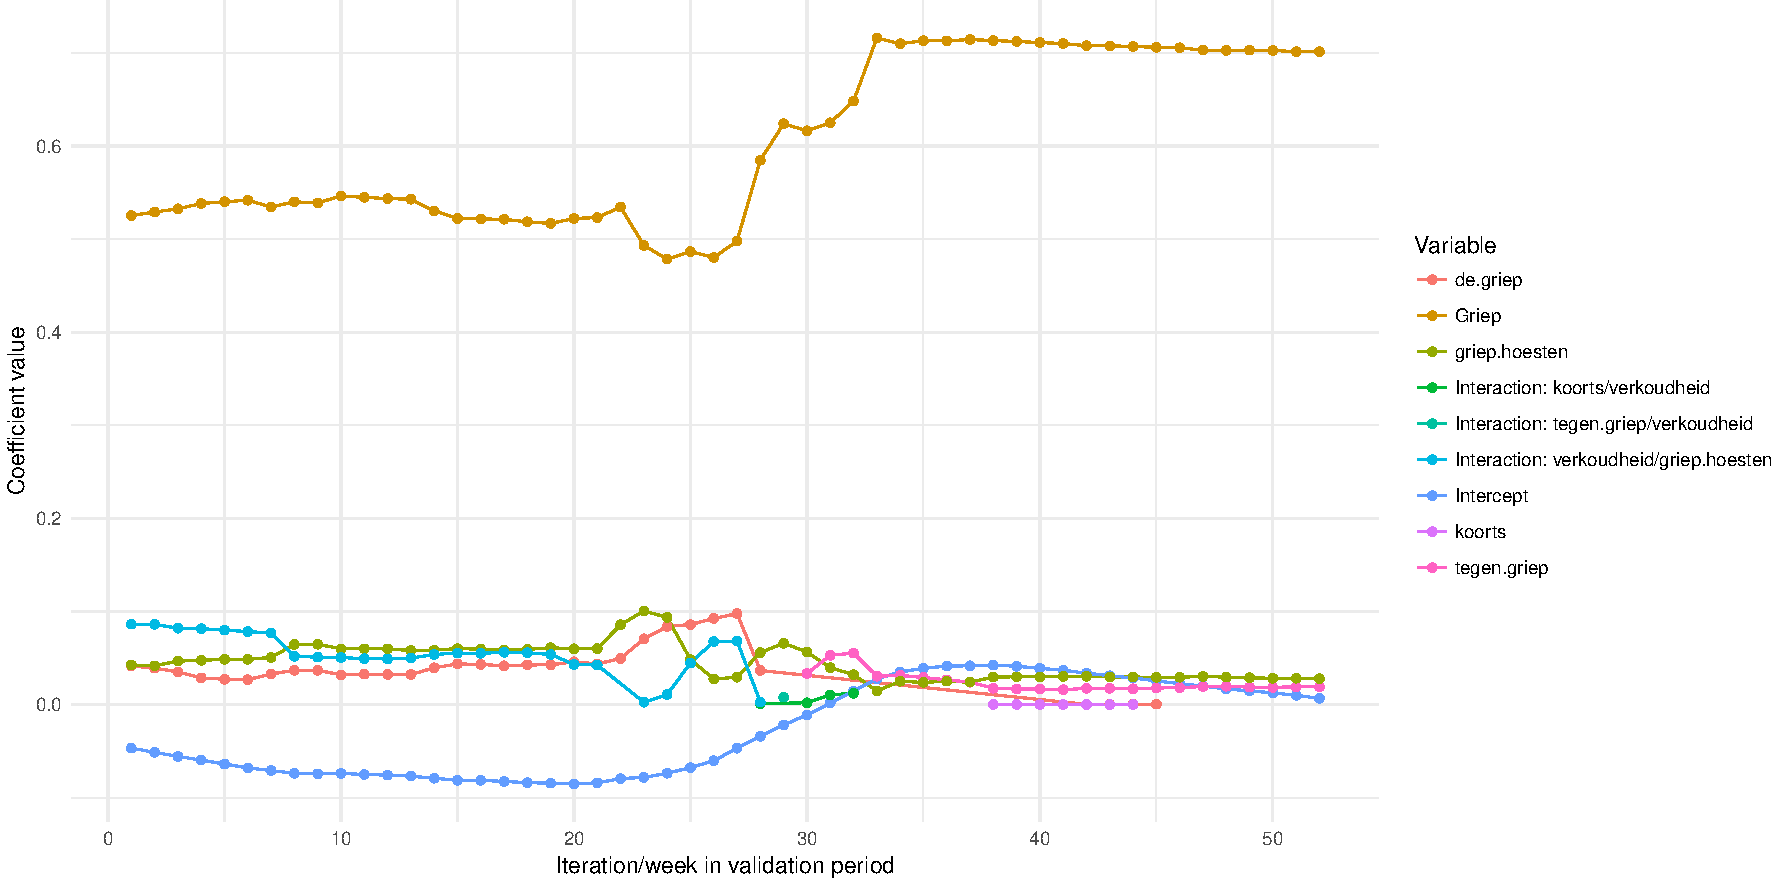
\includegraphics{unnamed-chunk-5-1.pdf}
\caption{Predictors retained in the final lasso regression models
throughout the 52 iterations. Coefficients with a value of zero are not
shown.}
\end{figure}

\hypertarget{discussion}{%
\subsection{\texorpdfstring{\textbf{Discussion}}{Discussion}}\label{discussion}}

Our study demonstrates that a statistical model, based on online search
queries, can be used to predict the ILI incidence in the Netherlands
during a normal influenza season. Assuming a four-week reporting lag,
our model predicted the 2017/18 ILI epidemic in real-time with
reasonable accuracy. The model would have identified the onset, peak,
and end of the epidemic with one to three weeks difference.

This investigation provides an accessible but rigorous case study in
digital epidemiology. The modelling steps are tractable and
computationally economical, so that the source code can be modified and
transferred to other settings. Indeed, we would encourage others to try
this method in other countries and other infectious diseases or outcomes
with a seasonal pattern (e.g.~hayfever, asthma).

A feature of our study, that is worth highlighting, is the week-by-week
simulation of the prediction model. We built 52 models, each of which
was validated on four weeks of data (which were later used for fitting
subsequent models). This iterative analysis loop allowed us to set a
realistic framework for investigating our research question. Our results
reflect how well a model would have performed, and what information it
would have provided if it was used during the 2017/18 ILI season. The
loop structure also enabled us to continuously update the model, as
suggested by previous research{[}6,16{]}, to prevent deterioration of
performance. Each week, we re-fitted the prediction model using the most
recently available ILI data from 4 weeks ago. We took this a step
further and also repetitively applied CV to select the momentarily
optimal set of predictors. Interestingly, most retained variables only
changed marginally over time, and one predictor (`Griep') had by far the
highest weight in all prediction models.

When preparing this project, we assessed a number of different data
sources (e.g.~Google searches and Wikipedia page visits),{[}8{]} but
chose the data from Google Trends{[}12{]} to be the most advantageous
for our project. The Google Trends service is publicly available, easy
to use, and it covers the online search behavior of a majority of people
in the Netherlands. It did come with certain limitations that should be
considered when interpreting our findings or applying this methodology.
Using the public API, weekly data can only be retrieved for periods of
less than five years, which sets a boundary for the observation period.
There is also a quota for the number of search requests, which limits
the amount of predictor data that can be downloaded. Moreover, we cannot
rule out that information was leaked from future to past observations,
since we retrieved all data after the end of the season. If the data
were retrieved each week during the season, results could have been
different.{[}17{]} This is a point that should be assessed in the
future.

In our modelling approach, we intentionally compromised on accuracy to
provide a fast and comprehensible model. To further improve the
predictive performance of our method, the model could be expanded by
adopting strategies that have been successfully applied in other
studies, including the use of more predictors (e.g.~unrelated search
queries and autoregressive terms){[}18{]}, additional data sources
(e.g.~Wikipedia page views, Twitter activity){[}19,20{]}, more extensive
data pre-processing (e.g.~principal component analysis), and alternative
statistical models (e.g.~ensemble methods){[}7,20{]}.

Our results are comparable to previous studies from European countries.
Valdivia et al.{[}21{]} used historic data from the now terminated
Google Flu Trends project and compared predicted ILI rates against
sentinel surveillance estimates across the 13 European countries during
the 2009/10 influenza pandemic. They found high correlations, with
Spearman coefficients ranging from .72 in Poland to .94 in Germany. For
the Netherlands, the authors report a correlation of .86, which is
slightly lower than what we found in our study ( = 0.90). More recently,
Samaras et al.{[}22{]} studied the association between ILI incidence and
influenza-related Google search queries in Greece and Italy in 2011 and
2012. They found Pearson correlation coefficients between .831 for
Greece and .979 for Italy. It should be noted, however, that these
figures were not validated on a test data set.

Numerous other studies, mostly from the US, have aimed to predict ILI
incidence rates from online data. They have used various data sources
and applied an array of different methods (Milinovich et al.{[}2{]} and
O'Shea et al.{[}7{]} provide informative overviews). Unfortunately, many
of the published studies suffer from methodological limitations, such as
the use of inappropriate outcome measures (e.g.~Spearman Rho), the
absence of a rigorous validation method (e.g.~using a single data set to
fit a model and evaluate its predictions), or insufficient reporting
(which does not allow for replication of results). Tabataba et
al.{[}23{]} and Generous et al.{[}24{]} have published in-depth
discussions of these points.

\hypertarget{implications-and-outlook}{%
\paragraph{\texorpdfstring{\textbf{Implications and
outlook}}{Implications and outlook}}\label{implications-and-outlook}}

In the Netherlands, there is no obvious case for monitoring ILI with
these methods. ILI data, including virological information, are
collected from sentinel practices on a weekly basis. However, during
weeks 52/2017 and 01/2018, we made an interesting observation: the
sentinel surveillance data indicated a temporary drop in the ILI
incidence but we find the signal was likely not to have been caused by a
decrease in the number of ILI cases, but rather by low health care
utilization and/or changes in doctors' working hours during the
Christmas/New Year holiday period. For these two weeks, it could be
argued that our prediction model could have usefully complemented the
sentinel surveillance system.

Further potential applications of this digital epidemiology method
include the provision of supportive low-cost online surveillance methods
in resource-poor countries (e.g.~countries which report data more slowly
than in the Netherlands or do not cover all regions of a country) and an
early warning system for pandemic outbreaks.{[}1{]} However, before
these novel methods can be used in routine practice, more research is
needed to better understand where, when, and how online surveillance can
complement established systems in all world regions. The value of
digital epidemiology still needs to be determined. To allow for
incremental learning, future studies should report methods in sufficient
detail, ideally providing the underlying source code and data.

\hypertarget{conclusions}{%
\subsection{\texorpdfstring{\textbf{Conclusions}}{Conclusions}}\label{conclusions}}

Our study demonstrates that a prediction model, based on online search
queries, could have predicted the 2017/18 ILI epidemic in the
Netherlands in real-time. The intensity of the epidemic, as well as its
onset, peak, and end were estimated with reasonable accuracy. The value
of using online surveillance methods to complement traditional disease
surveillance systems should be further explored.

\hypertarget{references}{%
\subsection{\texorpdfstring{\textbf{References}}{References}}\label{references}}

\hypertarget{refs}{}
\leavevmode\hypertarget{ref-Salathe2012}{}%
1. Salathe M, Bengtsson L, Bodnar TJ, Brewer DD, Brownstein JS, Buckee
C, et al. Digital epidemiology. PLoS computational biology.
2012;8(7):e1002616.

\leavevmode\hypertarget{ref-Milinovich2014}{}%
2. Milinovich GJ, Williams GM, Clements ACA, Hu W. Internet-based
surveillance systems for monitoring emerging infectious diseases. The
Lancet Infectious diseases. 2014 Feb;14(2):160--8.

\leavevmode\hypertarget{ref-Simonsen2016}{}%
3. Simonsen L, Gog JR, Olson D, Viboud C. Infectious Disease
Surveillance in the Big Data Era: Towards Faster and Locally Relevant
Systems. The Journal of infectious diseases. 2016
Dec;214(suppl\_4):S380--5.

\leavevmode\hypertarget{ref-Bovi2003}{}%
4. Bovi AM. Use of health-related online sites. The American journal of
bioethics : AJOB. 2003;3(3):W--IF3.

\leavevmode\hypertarget{ref-Ginsberg2009}{}%
5. Ginsberg J, Mohebbi MH, Patel RS, Brammer L, Smolinski MS, Brilliant
L. Detecting influenza epidemics using search engine query data. Nature.
2009 Feb;457(7232):1012--4.

\leavevmode\hypertarget{ref-Lazer2014}{}%
6. Lazer D, Kennedy R, King G, Vespignani A. Big data. The parable of
Google Flu: traps in big data analysis. Science (New York, NY). 2014
Mar;343(6176):1203--5.

\leavevmode\hypertarget{ref-OShea2017}{}%
7. O'Shea J. Digital disease detection: A systematic review of
event-based internet biosurveillance systems. International journal of
medical informatics. 2017 May;101:15--22.

\leavevmode\hypertarget{ref-PFT2017}{}%
8. Schneider P, Paget J, Spreeuwenberg P, Barnett D, Gool C van. Using
Wikipedia and Google data to estimate near real-time influenza incidence
in Germany: A Tutorial in R. 2018; Available from:
\url{https://projectflutrend.github.io/}

\leavevmode\hypertarget{ref-Nivel2018}{}%
9. Nivel. Netherlands Institute of Health Service Research. Primary care
database. 2018; Available from:
\url{http://www.nivel.nl/en/dossier/nivel-primary-care-database}

\leavevmode\hypertarget{ref-ECDC2018}{}%
10. ECDC. European Centre for Disease Prevention and Control. The
european surveillance system -- tessy. 2018; Available from:
\url{https://ecdc.europa.eu/en/publications-data/european-surveillance-system-tessy}

\leavevmode\hypertarget{ref-Donker2015}{}%
11. Donker GA. Nivel primary care database - sentinel practices 2015.
2016; Available from:
\url{https://www.nivel.nl/sites/default/files/bestanden/Peilstations_2015_Engel.pdf?}

\leavevmode\hypertarget{ref-GT2018}{}%
12. Google. Google trends. 2018; Available from:
\url{https://trends.google.com/trends/}

\leavevmode\hypertarget{ref-gtrendsR}{}%
13. Massicotte P, Eddelbuettel D. GtrendsR: Perform and display google
trends queries. 2018. Available from:
\url{https://github.com/PMassicotte/gtrendsR}

\leavevmode\hypertarget{ref-Tibshirani1996}{}%
14. Tibshirani R. Regression shrinkage and selection via the lasso.
Journal of the Royal Statistical Society Series B. 1996;58(1):267--88.

\leavevmode\hypertarget{ref-repository}{}%
15. Schneider P, Gool C van, Spreeuwenberg P, Barnett D, Paget J. Using
digital epidemiology methods to monitor influenza-like illness in the
netherlands in real-time: Source code \& data repository. Github
repository. 2018; Available from:
\url{https://github.com/bitowaqr/DutchFluTrend}

\leavevmode\hypertarget{ref-Santillana2014}{}%
16. Santillana M, Zhang DW, Althouse BM, Ayers JW. What can digital
disease detection learn from (an external revision to) Google Flu
Trends? American journal of preventive medicine. 2014 Sep;47(3):341--7.

\leavevmode\hypertarget{ref-Jun2018}{}%
17. Jun S-P, Yoo HS, Choi S. Ten years of research change using Google
Trends: From the perspective of big data utilizations and applications.
Technological Forecasting and Social Change. 2018;130:69--87.

\leavevmode\hypertarget{ref-Preis2014}{}%
18. Preis T, Moat HS. Adaptive nowcasting of influenza outbreaks using
Google searches. Royal Society open science. 2014 Oct;1(2):140095.

\leavevmode\hypertarget{ref-McIver2014}{}%
19. McIver DJ, Brownstein JS. Wikipedia usage estimates prevalence of
influenza-like illness in the United States in near real-time. PLoS
computational biology. 2014 Apr;10(4):e1003581.

\leavevmode\hypertarget{ref-Santillana2015}{}%
20. Santillana M, Nguyen AT, Dredze M, Paul MJ, Nsoesie EO, Brownstein
JS. Combining Search, Social Media, and Traditional Data Sources to
Improve Influenza Surveillance. PLoS computational biology. 2015
Oct;11(10):e1004513.

\leavevmode\hypertarget{ref-Valdivia2010}{}%
21. Valdivia A, Lopez-Alcalde J, Vicente M, Pichiule M, Ruiz M, Ordobas
M. Monitoring influenza activity in Europe with Google Flu Trends:
comparison with the findings of sentinel physician networks - results
for 2009-10. Euro surveillance : bulletin Europeen sur les maladies
transmissibles = European communicable disease bulletin. 2010
Jul;15(29).

\leavevmode\hypertarget{ref-Samaras2017}{}%
22. Samaras L, Garcia-Barriocanal E, Sicilia M-A. Syndromic Surveillance
Models Using Web Data: The Case of Influenza in Greece and Italy Using
Google Trends. JMIR public health and surveillance. 2017 Nov;3(4):e90.

\leavevmode\hypertarget{ref-Tabataba2017}{}%
23. Tabataba FS, Chakraborty P, Ramakrishnan N, Venkatramanan S, Chen J,
Lewis B, et al. A framework for evaluating epidemic forecasts. BMC
infectious diseases. 2017 May;17(1):345.

\leavevmode\hypertarget{ref-Generous2014}{}%
24. Generous N, Fairchild G, Deshpande A, Del Valle SY, Priedhorsky R.
Global disease monitoring and forecasting with Wikipedia. PLoS
computational biology. 2014 Nov;10(11):e1003892.


\end{document}
